\documentclass[11pt]{article}
%\documentclass[preprint, 10pt]{elsarticle}

% PACKAGES
\usepackage{graphicx, amsmath, amssymb, amsfonts, mathtools, mathrsfs, color}
\usepackage{comment, enumerate, tabularx}
\usepackage{natbib, hyperref, url}
\usepackage[margin=1in]{geometry}
%\usepackage[justification=RaggedRight]{caption}

%----------------------------------------------------------------------------%
%% LATEX DEFINITIONS
%----------------------------------------------------------------------------%
% Basic editing
\newcommand{\tocite}{{\color{blue}(to cite)}}
\newcommand{\vsp}[1]{\vspace{#1 pc} \noindent}
\newcommand{\np}{\newpage \noindent}
% Derivatives
\newcommand{\pd}[2]    { \frac{\partial #1} {\partial #2} }
\newcommand{\ppd}[2]  { \frac{\partial^2 #1}{{\partial #2}^2} }
\newcommand{\pdi}[2] { {\partial_#2} #1 }
\newcommand{\td}[2] { \frac{d #1} { d #2 } }
\newcommand{\grad}{\nabla}
\newcommand {\Lap} {\grad^2}
% Vectors and operators
\newcommand{\bvec}[1]{\ensuremath{\boldsymbol{#1}}}
\newcommand{\abs}[1]{\left| #1 \right|}
\newcommand{\norm}[1]{\left\| #1 \right\|}
\newcommand{\mean}[1]{\left< #1 \right>}
\newcommand{\eps}{\varepsilon}
\newcommand{\dx}{\, dx}
% Basic physical parameters and scales
\newcommand{\freqp}{f_p}
\newcommand{\etastd}{\eta_{\text std}}
% Parameters that change crossing the ADC
\newcommand{\depth}{d}
\newcommand{\dup}{\depth_{-}}
\newcommand{\ddn}{\depth_{+}}
\newcommand{\dupdn}{\depth_{\pm}}
\newcommand{\lam}{\lambda}
\newcommand{\lamup}{\lam_{-}}
\newcommand{\lamdn}{\lam_{+}}
\newcommand{\lamupdn}{\lam_{\pm}}
\newcommand{\lamfac}{N}
\newcommand{\drat}{\mathcal{D}}
\newcommand{\dratdn}{\drat_+}
\newcommand{\dratupdn}{\drat_{\pm}}
% Statistical quantities
\newcommand{\En}{\mathcal{E}}
\newcommand{\Mo}{\mathcal{M}}
\newcommand{\skw}{\text{skew}}
\newcommand{\skwdn}{\skw_+}
\newcommand{\var}{\text{var}}
\newcommand{\varup}{\var_-}
\newcommand{\vardn}{\var_+}
% Dimensionless parameters
\newcommand{\ampscale}{\mathcal{A}}
\newcommand{\lengthscale}{\mathcal{L}}
\newcommand{\timescale}{\mathcal{T}}
\newcommand{\epsup}{\eps_0}
\newcommand{\delup}{\delta_0}
% Hamiltonian stuff
\newcommand{\uhat}{\hat{u}}
\newcommand{\sympJ}{\mathcal{J}}
\newcommand{\vard}[2]{\frac{\delta #1}{\delta #2}}
\newcommand{\Ham}{\mathcal{H}}
\newcommand{\Hup}{\Ham^{-}}
\newcommand{\Hdn}{\Ham^{+}}
\newcommand{\Hupdn}{\Ham^{\pm}}
\newcommand{\Hthree}{\Ham_{3}}
\newcommand{\Htwo}{\Ham_{2}}
%\newcommand{\Fcnl}{\mathcal{F}}
% Truncated stuff
\newcommand{\Proj}{\mathcal{P}_{\Lambda}}
\newcommand{\uL}{u_{\Lambda}}
\newcommand{\HLupdn}{\Ham_{\Lambda}^{\pm}}
\newcommand{\SympL}{\sympJ_{\Lambda}}
\newcommand{\uup}{u_{-}}
\newcommand{\udn}{u_{+}}
\newcommand{\uupdn}{u_{\pm}}
% Gibbs and theta
\newcommand{\Gibbs}{\mathcal{G}}
\newcommand{\Gup}{\Gibbs^{-}}
\newcommand{\Gdn}{\Gibbs^{+}}
\newcommand{\Gupdn}{\Gibbs^{\pm}}
\newcommand{\thup}{\theta^{-}}
\newcommand{\thdn}{\theta^{+}}
\newcommand{\thupdn}{\theta^{\pm}}
\newcommand{\meanup}[1]{\mean{#1}_{-}}
\newcommand{\meandn}[1]{\mean{#1}_{+}}
\newcommand{\meanupdn}[1]{\mean{#1}_{\pm}}
\newcommand{\tavg}[1]{\overline{#1}}
\newcommand{\transf}{\mathcal{F}}

% Experiments
\newcommand{\omavg}{\omega_0}
\newcommand{\omsig}{\sigma_{\omega}}
\newcommand{\Dphi}{\Delta \phi}

%----------------------------------------------------------------------------%

%----------------------------------------------%
%% TITLE
%----------------------------------------------%
\begin{document}

\title{Anomalous waves triggered by abrupt depth changes: experimental measurements and deterministic-statistical truncated KdV theory}

% ORIGINAL: The truncated KdV framework for modeling anomalous waves induced by abrupt depth changes
% Words: triggered, induced, generated, sparked

\author{
C.~Tyler Bolles\thanks{University of Michigan},
Andrew J.~Majda\thanks{Courant Institute of Mathematical Sciences}, 
M.~N.~J.~Moore\thanks{Florida State University}, 
Di Qi\thanks{Courant Institute of Mathematical Sciences} }
\maketitle

\begin{abstract} 
Recent laboratory experiments revealed the emergence of anomalous statistics in a randomized surface waves upon encountering an abrupt depth change (ADC) in the bottom topography (Bolles et al. PRF 2019). Majda et al.~2019 established a theoretical foundation, based on analysis of the truncated KdV (TKdV) system, that successfully captures several key qualitative features of the experiments including the robust emergence of anomalous statistics. The framework exploits the Hamiltonian structure of TKdV to construct invariant measures that are statistical matched at the ADC, and is corroborated by simulations of the deterministic dynamics. 
%
Here we present a more comprehensive treatment of these parallel experimental and modeling efforts, with emphasis on the link between the two. We present an assortment of new experimental measurements and carefully compare them to model predictions. We establish a more precise link between experimental and model parameters, so that the invariant measure underlying the model can be calibrated to the specific conditions present in experiments. The model predicts a peculiar relationship between surface-displacement skewness and surface-slope variance, which is confirmed in spectacular fashion by direct experimental measurements.
\end{abstract}


%----------------------------------------------------------%
% Intro
%----------------------------------------------------------%
\section{Introduction}

Rogue waves are abnormally large surface waves, defined by oceanographers as those that exceed twice the significant wave height \citep{muller2005rogue, ying2011linear}. Though such waves were once dismissed as myth, they have now been recorded in oceans across the globe and pose a recognized threat to seagoing vessels and naval structures. Rogue waves, also variously known as freak or anomalous waves, have been observed both in deep and shallow water, and can be triggered by a variety of mechanisms, including anomalous wind-forcing \citep{kharif2008influence, toffoli2017wind}, 
focusing due to variable bathymetry \citep{heller2008refraction, white1998chance}, 
opposing currents \citep{garrett2009rogue, onorato2011triggering},
and the Benjamin-Feir deep-water modulational instability \citep{benjamin1967disintegration, viotti2013emergence, cousins2015unsteady, farazmand2017reduced}.
The common tie between these mechanisms is their ability to generate non-normal statistics in the surface displacement; when governed by Gaussian statistics, the likelihood of a rogue wave is extremely low, but these rare events occur much more frequently when surface statistics deviate from Gaussian. In this way, it makes sense to approach anomalous waves from the broader perspective of turbulent dynamical systems \cite{sapsis2013a, sapsis2013b, sapsis2013blending, chen2016filtering, majda2016introduction, macedo2017universality, MajdaQiSIAM2018, blonigan2019extreme, guth2019machine}.

A recent series of laboratory \cite{bolles2019} and numerical investigations \cite{viotti2014} have demonstrated the emergence of anomalous wave statistics from abrupt variations in bottom topography. Since topographical variations are strictly one-dimensional, these studies can be viewed as offering a bare minimum set of conditions capable of generating anomalous wave statistics. In particular, the more complex mechanism of focusing by 2D bottom topography absent. The studies thus offer a paradigm system, with emergent anomalous statistical properties similar to that seen in more complex systems, but in a tractable context that is amenable to analysis.

Our particular focus is the laboratory experiments of Bolles et al.~\cite{bolles2019}, who demonstrated the emergence of anomalous statistics from a randomized wave-field encountering an abrupt depth change (ADC). In these experiments, the incoming wave-field is generated with nearly Gaussian statistics, and a plexiglass step placed near the middle of the tank creates the depth change. Upon passing into the shallower region, the wave distribution skews strongly towards positive displacement, with deviation from Gaussian being most pronounced a short distance downstream of the ADC. Inspired by these experimental observations, Majda et al.~\cite{majda2019} developed a theoretical framework that accurately captures several key aspects of the anomalous behavior. The theory is based on deterministic and statistical analysis of the truncated Korteweg–de Vries (TKdV) equations, and uses a combination of computational, statistical, and analytical tools. In follow-up work, Majda and Qi \cite{majdaqi2019} analyzed more severely truncated systems of lower dimension that were shown to exhibit many of the same anomalous properties while enjoying a more tractable structure.

The purpose of the present manuscript is to provide a more comprehensive treatment of the {\em combined} experimental and theoretical efforts of Bolles et al~\cite{bolles2019} and Majda et al.~\cite{majda2019, majdaqi2019}. Special emphasis is placed on the synergy between experiment and theory -- a cooperative strategy with a proven record of success \cite{camassa2012stratified, ristroph2012, ganedi2018equilibrium}. We present an assortment of previously unpublished experimental data, for example on surface slope statistics and autocorrelation, which motivates further examination and refinement of the theory. Likewise, novel theoretical predictions have inspired us to perform additional experimental measurements, particularly regarding a peculiar relationship between surface-displacement skewness and surface-slope variance that is predicted by the theory. Comparison with the new measurements further confirms the predictive power of the framework developed by Majda et al.~\cite{majda2019}. In addition, we provide a more thorough treatment of the link between experimental and model parameters to facilitate comparison between the two. In particular, we flesh out details of non-dimensionalization, which were only briefly addressed in prior work for the sake of brevity.

% Words: conjunction, combination, close cooperation; elucidate.
% New data: slopes, autocorrelation, depth ratio varied.


%----------------------------------------------------------%
% Experiments
%----------------------------------------------------------%
\section{The experiments}

	As diagrammed in Fig.~\ref{ExpDiagStats}(a), the experiments consist of a long, narrow wave tank (6 m long x 20 cm wide x 30 cm high), with waves generated by plexiglass paddle at one end \cite{bolles2019}. The waves propagate through the tank and, roughly midway through, pass over an abrupt depth change (ADC) created by a plexiglass step. The waves continue to propagate through the shallower depth until reaching the far end of the tank, at which point their energy is dissipated by a horse-hair dampener. Since the dampener minimizes backscatter, the waves in this experiment propagate primarily in one direction, from left to right in Fig.~\ref{ExpDiagStats}(a). 

The pivoting motion of the paddle is driven by a 5-phase stepper motor. To generate a randomized incoming wave field, the paddle angle $\phi$ is specified by a precomputed psuedo-random signal
\begin{align}
\label{PaddleAngle}
& \phi(t) = \phi_0 + \Dphi \sum_{n=1}^N a_n \cos(\omega_n t+\delta_n) \, , \\
\label{anEq}
& a_n = \sqrt{\frac{2 \Delta \omega}{\pi^{1/2} \omsig}} \, 
\exp \left( -\frac{(\omega_n - \omavg)^2}{2 \omsig^2} \right) \, ,
\end{align}
The angular frequencies are evenly spaced $\omega_n = n  \Delta \omega$ with step size $ \Delta \omega = (\omavg+4 \omsig)/N$, where $\omavg$ and $\omsig$ represent the mean and the bandwidth of $\omega$ respectively. As in prior work, all experiments reported here use the values $\omavg = \omsig = 12.5$ rad/s, corresponding to a peak forcing frequency of 2 Hz and bandwidth of 2 Hz. Meanwhile, the phases $\delta_n$ are uniformly distributed random variables. The standard deviation of the paddle angle, $\Dphi$, controls the amplitude of the generated waves. In a single experiment $\Dphi$ is fixed, and we will present a series of experiments with systematically varied values of $\Dphi$.

% Figure: Experimental Diagram and Histograms
%^^^^^^^^^^^^^^^^^^^^^^^^^^^^^^%
\begin{figure}%[!ht]
\begin{center}
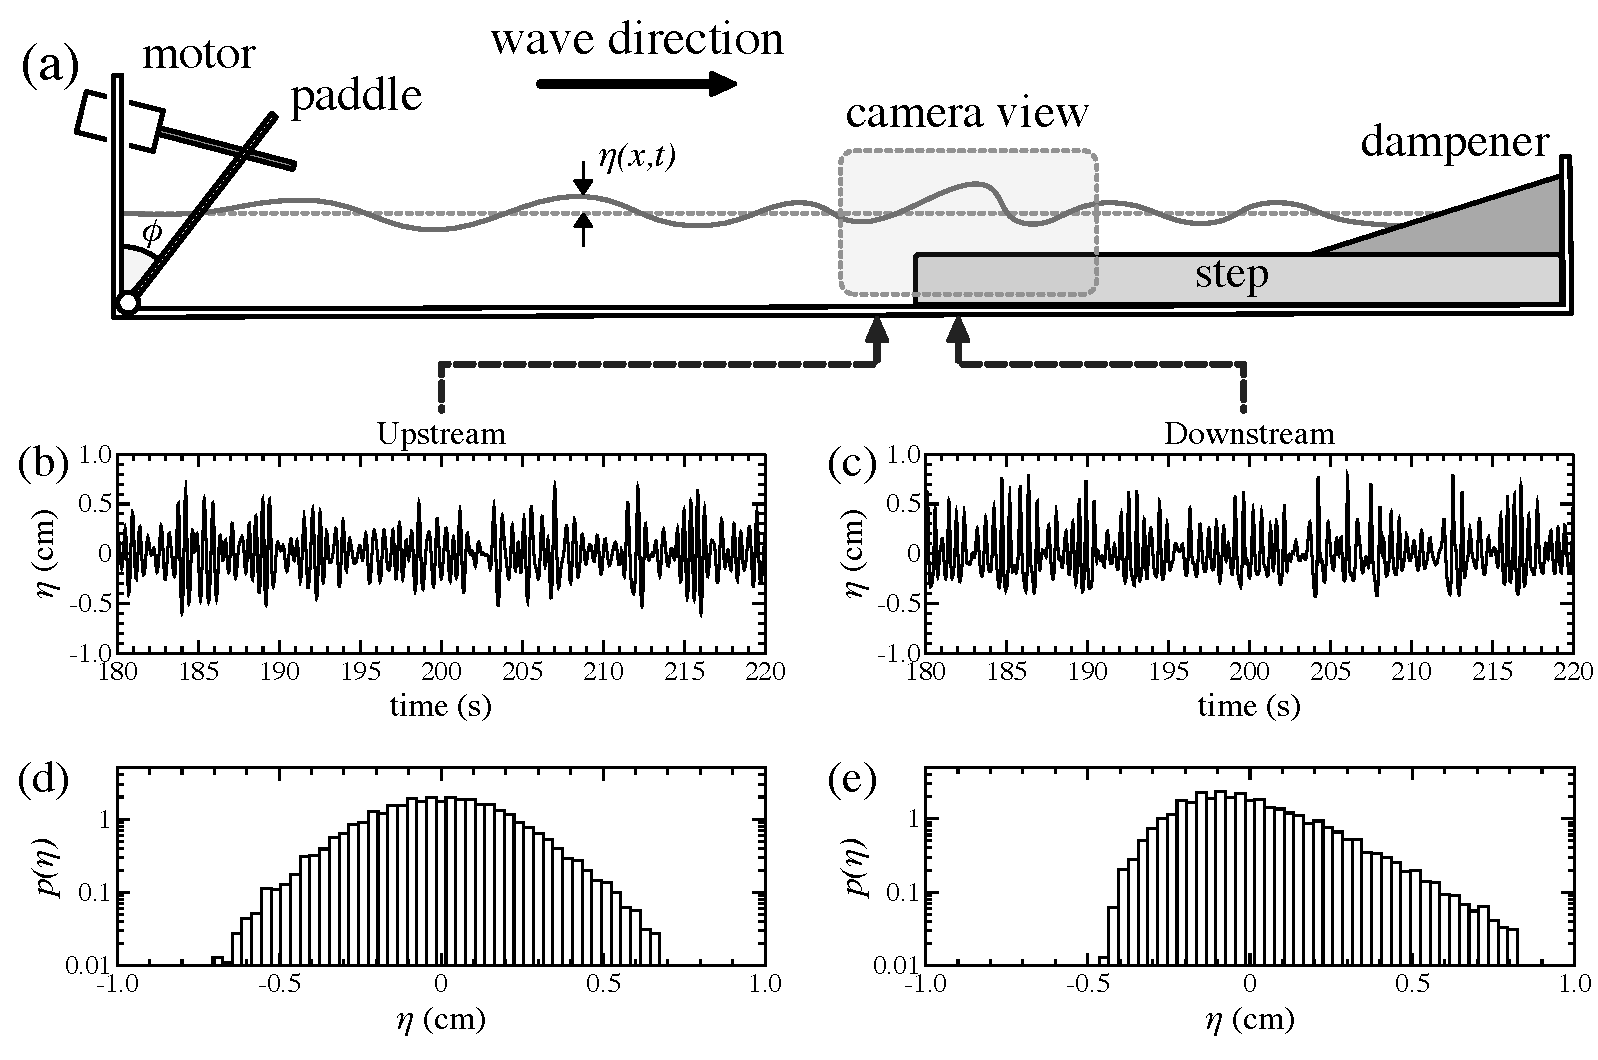
\includegraphics[width = 0.85 \linewidth]{Figs/ExpDiagStats.pdf}
\caption{
(a) Experimental schematic. 
(b)--(c) Surface displacement measured at a representative upstream and downstream locations. (d)--(e) Corresponding histograms. Figure adapted from \cite{bolles2019}.}
\label{ExpDiagStats}
\end{center}
\end{figure}
%^^^^^^^^^^^^^^^^^^^^^^^^^^^^^^%
% Data from column 5 in MasterTimeSeries, Delta theta = 1.38 degrees, which is in between runs 5 and 6.
 
	The free surface is illuminated by light-emitting diodes running along the bottom of the tank and is imaged from the sideview with a Nikon D3300 at 60 frames per second. The illumination technique, coupled with high pixel count of the camera, allows surface displacements to be resolved with accuracy better than 1/3 millimeter. Furthermore, these optical measurements permit extraction of wave statistics {\em continuously} in space, rather than at a few discrete locations, which is crucial for identifying regions of anomalous wave activity. Further details of the experimental setup can be found in \cite{bolles2019}.

	Example measurements of free-surface displacements $\eta$ are shown in Figs.~\ref{ExpDiagStats}(b)--(c). These measurements are extracted from the images at two representative locations: one a short distance (9 cm) upstream of the ADC and the other (15 cm) downstream of the ADC. Both signals exhibit a combination of periodic behavior and random fluctuations, with the dominant oscillations corresponding to the peak driving frequency of 2 Hz. The nature of the random fluctuations is revealed by the corresponding histograms shown in Fig.~\ref{ExpDiagStats}(d)--(e). The upstream measurements are symmetrically distributed about the mean, $\eta = 0$. In fact, Bolles et al.~found that these measurements follow a Gaussian distribution closely \cite{bolles2019}. The downstream measurements, however, are not symmetrically distributed and skew strongly towards positive displacement, $\eta > 0$. Bolles et al.~found that these measurements can be well described by a mean-zero gamma distribution \cite{bolles2019}. The slower decay rate of this downstream distribution indicates an elevated level of extreme surface displacement, i.e.~rogue waves. Bolles et al.~estimated that a rogue wave can be up to 65 times more likely in these experiments than if the displacements were Gaussian. 

	The measurements shown in Fig.~\ref{ExpDiagStats} correspond to a paddle driving amplitude of $\Dphi = 1.38^{\circ}$, an upstream depth of $\dup = 12.5$ cm, and a downstream depth of $\ddn = 3$ cm, which gives the depth ratio $\dratdn = \ddn/\dup= 0.24$. Bolles et al.~systematically varied the driving amplitude in the range $0.125^{\circ}$--$2^{\circ}$ to probe different regimes of wave behavior, from nearly linear waves to strongly nonlinear ones. They found that once a critical amplitude is exceeded (roughly $\Dphi = 0.5^{\circ}$), the downstream statistics become anomalous and are robustly described by the gamma-distribution. Fig.~\ref{ExpSpatialStats} shows spatial statistics for several experiments of different driving amplitudes. The standard deviation of surface displacement $\etastd$ measures the characteristic amplitude of waves (Fig.~\ref{ExpSpatialStats}(a)). Notice that $\etastd$ increases with paddle amplitude, but does not significantly vary in space. In particular, $\etastd$ does not change significantly when waves cross the ADC. Skewness and (excess) kurtosis, however change markedly crossing the ADC once the critical driving amplitude is exceeded. We also show statistics of surface slope $\eta_x$.

 % Figure: Experimental Spatial Statistics
%^^^^^^^^^^^^^^^^^^^^^^^^^^^^^^%
\begin{figure}%[!ht]
\begin{center}
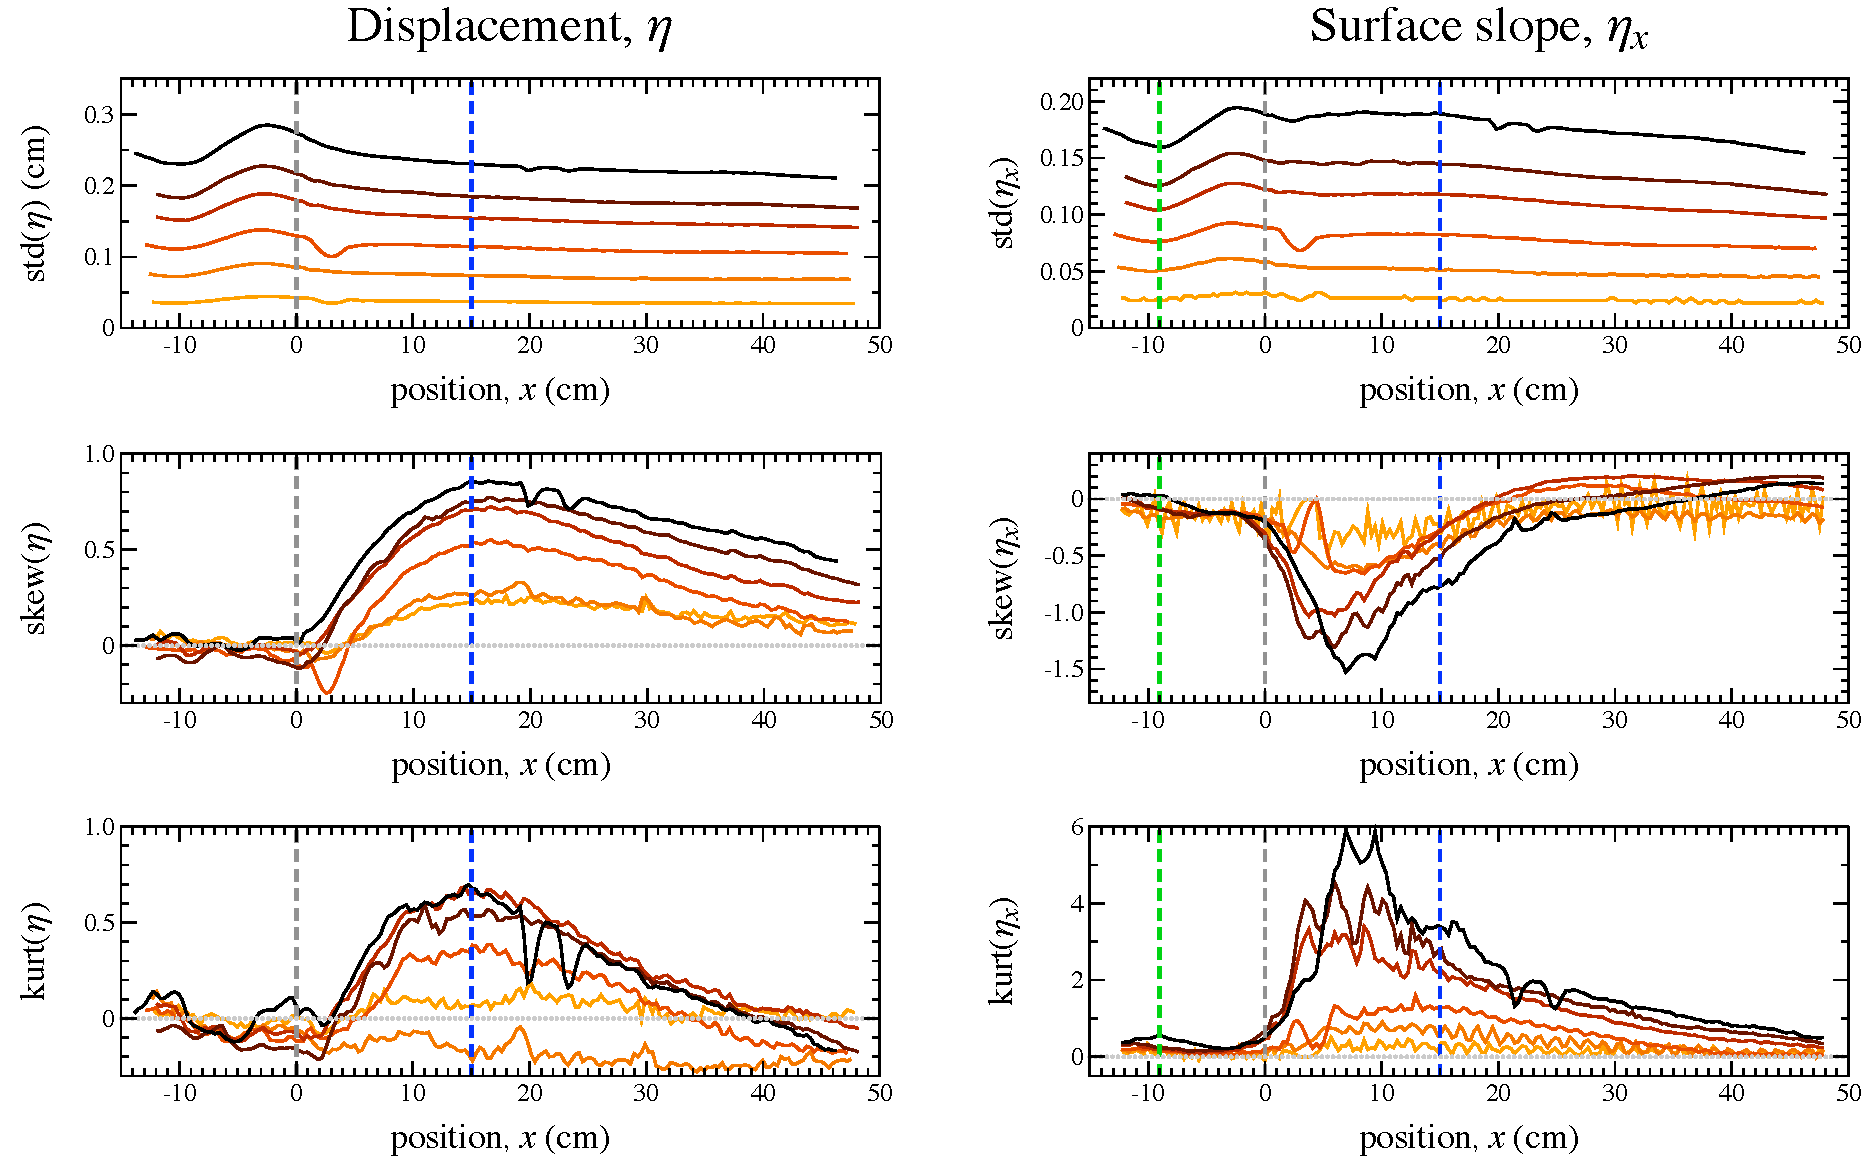
\includegraphics[width = 0.9 \linewidth]{Figs/ExpSpatialStats.pdf}
\caption{Wave statistics as they vary in space for several different experiments of different driving amplitudes (see legend). $\etastd$ does not vary significantly crossing the ADC (a), but skewness (b) and kurtosis (c) show a strong response to the ADC. }
\label{ExpSpatialStats}
\end{center}
\end{figure}
 %^^^^^^^^^^^^^^^^^^^^^^^^^^^^^^%

	Bolles et al.~systematically explored the effect of varying the driving amplitude on the anomalous statistics for a fixed depth ratio. Here, we further explore the effect of driving amplitude, especially in conjunction with theoretical developments, and we will also report experiments in which the depth ratio was varied. We will refer to the experiments displayed in Fig.~\ref{ExpDiagStats} as the reference experiments, so that we have a baseline for comparison. In these reference experiments, the driving amplitude is $\Dphi = 1.38^{\circ}$ (intermediate between the cases $\Dphi = 1.25^{\circ}$ and $1.5^{\circ}$ shown in Fig.~\ref{ExpDiagStats}(a)), the depth ratio is $\dratdn = 0.24$, and the characteristic wave amplitude is $\etastd = 0.21$ cm.

%$\epsup = 0.017$.





 
%----------------------------------------------------------%
% Theory
%----------------------------------------------------------%
\section{Theoretical framework}

We now introduce the theoretical framework that will be used to understand and quantify the experimental observations. This framework is based on a Galerkin truncation of the variable-depth Korteweg–de Vries (KdV) equation. The KdV equation is a commonly excepted model for describing the propagation of unidirectional, shallow-water waves, accounting for weak nonlinearity and weak dispersion over long timescales and large spatial scales. We will perform Galerkin truncation of this system at wavenumber $\Lambda = $8--32 to obtain a finite dimensional dynamical system exhibiting weak turbulence. We outline the Hamiltonian structure of both the continuous KdV and the truncated system. This structure is exploited to obtain invariant measures of the underlying dynamics and to ultimately understand the experimental findings on anomalous wave statistics triggered by an ADC.


%----------------------------------------------------------------------------%
% KdV
%----------------------------------------------------------------------------%
\subsection{The Korteweg–de Vries equation with variable depth}
Consider waves propagating unidirectionally in shallow water. Consider the surface displacement $\eta(x,t)$ and the reference frame moving with the local wave speed $\xi = x - ct$, where $c = \sqrt{g \depth}$ is the wave speed, $g$ gravity, and $\depth$ the local depth.
To first-correction in small amplitude, surface displacements are governed by the Korteweg–de Vries equation (KdV), which in dimensional form is given by \cite{whitham2011linear}
\begin{equation}
\label{KdV}
\eta_t + \frac{3 c}{2 \depth} \eta \eta_{\xi} + \frac{c \depth^2}{6} \eta_{\xi \xi \xi} = 0
\end{equation}
% This dimensional form is given by Whitham on p. 461, Eq. 13.98. I first got it from the Wolfram KdV, which gives the same equation.

As in the experiments, we consider waves that originate from a region of constant depth, encounter an abrupt depth change, and continue in another region of constant depth. Thus, depth will be piecewise constant
\begin{align}
\depth = 
\begin{cases}
\dup \quad \mbox{if } x<0 \\
\ddn \quad \mbox{if } x>0
\end{cases}
\end{align}
Most often, we will consider waves moving into shallower depth, so that $\dup > \ddn$. 

The incoming waves are randomized and generated with a peak forcing frequency of $\freqp$, which gives rise to the following quantities
\begin{align}
&c = \sqrt{g \depth}
&&\mbox{\em local wave speed} \\
&\lam = c/\freqp = \sqrt{g \depth} / \freqp
&&\mbox{\em local peak wave length} \\
&\etastd = \mean{\eta^2}^{1/2} 
&&\mbox{\em standard deviation of displacement} \\
\end{align}
where $\mean{\cdot}$ indicates the mean of a quantity. 
Note that the characteristic wave speed $c = c_{\pm}$ and wavelength $\lam = \lamupdn$ each take different values upstream and downstream of the ADC. We remark that experimental measurements indicate that $\etastd = \mean{\eta^2}^{1/2}$ is nearly the same on both values of the ADC. Hence, we will not distinguish between upstream and downstream values of $\etastd$.
%
See Table \ref{paramtable} for a summary of important parameters.

% Table
%^^^^^^^^^^^^^^^^^^^^^^^^^^^^^^%
\begin{table}[h]%[htbp]
\begin{center}
\caption{Table of parameters}
\label{paramtable}
\begin{tabular}{l l l}
\hline \multicolumn{3} { c }{Parameters that are constant in a single experiment} \\
\hline Description & Notation and definition & Value in experiments \\
\hline
Peak forcing frequency		& $f_p$						& 2 Hz \\
Characteristic wave amplitude	& $\etastd = \mean{\eta^2}^{1/2} $		& 0.03--0.3 cm \\
Upstream depth			& $\dup$						& 12.5 cm \\
Downstream depth			& $\ddn$						& 3 cm (and varied) \\
Upstream wavelength		& $\lamup = \sqrt{g \dup}/f_p$		& 55 cm \\
Upstream wavelength		& $\lamdn = \sqrt{g \ddn}/f_p$		& 27 cm \\
%
Amplitude-to-depth ratio		& $\epsup = \etastd / \dup$			& 0.0024--0.024 \\
Depth-to-wavelength ratio		& $\delup = \dup / \lamup$		& 0.22 \\
Depth ratio				& $\dratdn = \ddn/\dup$			& 0.24 (and varied)
\end{tabular}
\end{center}
\end{table}
 %^^^^^^^^^^^^^^^^^^^^^^^^^^^^^^%
 
 
%----------------------------------------------------------------------------%
% Nondimensionalization
%----------------------------------------------------------------------------%
\subsection{Nondimensionalization and relation to experimental scales}

In this section, the variable-depth KdV equation \eqref{KdV} will be recast into a dimensionless form chosen for convenience in working with the statistical-mechanics framework introduced in \cite{majda2019}. Since the choice of normalization not unique, it is instructive to first introduce a generic normalization to facilitate comparison with other choices. To this end, consider characteristic scales, $\ampscale, \lengthscale, \timescale$ for the wave amplitude, longitudinal length, and time respectively, which can remain unspecified for the moment. We introduce the dimensionless variables
\begin{align}
&u = \eta / \ampscale
&&\mbox{\em dimensionless surface displacement} \\
&\tilde{x} = \xi / \lengthscale
&&\mbox{\em dimensionless position (in moving frame)} \\
&\tilde{t} = t / \timescale
&&\mbox{\em dimensionless time}
\end{align}
Recasting \eqref{KdV} in terms of these variables gives the generic dimensionless KdV equation:
\begin{equation}
u_t + \frac{3}{2} \left( \frac{c \timescale \ampscale}{\lengthscale \depth} \right) u u_x 
+ \frac{1}{6} \left( \frac{c \timescale \depth^2}{\lengthscale^3} \right) u_{xxx} = 0
\end{equation}
We have dropped the tilde notation above for simplicity and will henceforth use tildes only in cases of possible ambiguity.

Now it is possible to choose the scales $\ampscale, \lengthscale, \timescale$ for ease in working with a particular framework. We choose the following scales,
\begin{align}
\label{scales}
\ampscale = \pi^{1/2} \, \etastd \, , \qquad
\lengthscale = \frac{\lamfac \lam}{2 \pi} \, , \qquad
\timescale = \frac{\lamfac \lam}{2 \pi \freqp \depth}
\end{align}
where $\lamfac$ is an integer to be chosen later. 
The explanation for these choices is as follows. First, we have chosen the characteristic amplitude, $\ampscale$, above to normalize the energy of the state-variable $u$ to unity, as will be demonstrated in Section \ref{tKdVSec}. Second, regarding $\lengthscale$, recall that $\lam$ is the characteristic wavelength corresponding to the peak forcing frequency $\freqp$ in the experiments. If only integer multiples of $\freqp$ were imposed (e.g.~lower frequencies were not present), then the forcing would produce waves that are periodic over lengthscale $\lam$. Since lower frequencies do exist, strict periodicity is not satisfied, but rather waves may be nearly periodic over the physical domain $\xi \in [-\lam/2, \lam/2]$. The approximation of near-periodicity becomes more accurate if integer multiples of $\lam$ are considered, i.e.~$\xi \in [-\lamfac \lam/2, \lamfac \lam/2]$. Thus, we have chosen $\lengthscale$ above so that the dimensionless domain of consideration is $\tilde{x} \in [-\pi, \pi]$ and periodic boundary conditions on $u$ can be  imposed on over this domain with accuracy that increases with $\lamfac$. Lastly, regarding $\timescale$, the most basic timescale in the experiments is simply $\freqp^{-1}$, i.e.~the period of waves passing a fixed reference point. Of course, the leading-order behavior in shallow water is simple translation of waves with uniform speed $c$. The KdV equation provides the first correction to this behavior and describes dynamics that evolve over longer timescales. Hence we have rescaled $\freqp^{-1}$ by the factor $N \lam/(2 \pi \depth) \gg 1$, which provides a suitably long timescale and is in line with previous normalizations \cite{johnson1997modern}. The scales $\lengthscale$ and $\timescale$ change value across the ADC, which is important to note when comparing the theory against experimental measurements.

With the above choices, the dimensionless KdV takes the form
\begin{align}
\label{dimlessKdV}
&u_t + C_3 \drat^{-3/2} \, u u_x + C_2 \drat^{1/2} \, u_{xxx} = 0
\qquad \text{for } x \in [-\pi,\pi] \\
&C_3 = \frac{3}{2} \pi^{1/2} \epsup \delup^{-1} \, , \quad
C_2 = \frac{2 \pi^2 \delup}{3 \lamfac^2} 
%C_2 = \frac{\pi^2 \delup}{6 \lamfac^2} 
\end{align}
The constants $C_3$ and $C_2$ do {\em not} change value crossing the ADC and are given in terms of the dimensionless parameters
\begin{align}
&\epsup = \etastd / \dup
&&\mbox{\em upstream amplitude-to-depth ratio} \\
&\delup = \dup / \lamup
&&\mbox{\em upstream depth-to-wavelength ratio}
\end{align}
The reason for the subscripts $3$ and $2$ will become evident in the next section. 

Meanwhile, the dimensionless depth $\drat = {\depth}/{\dup}$ {\em does} change value across the ADC since the depth $\depth$ changes. Recall that the reference frame of \eqref{dimlessKdV} moves with the local wave speed via the variable $\xi = x-ct$ from \eqref{KdV}. Thus, the ADC is met at some time $T_{ADC}$, and for simplicity we set $T_{ADC} = 0$. Therefore, we can regard $\drat$ is a piece-wise constant function of dimensionless time
\begin{equation}
\label{dratpw}
\drat = 
\begin{cases}
1 		&\quad \mbox{for } {t}<0 \\
\dratdn = {\ddn}/{\dup} 	&\quad \mbox{for } {t}>0
\end{cases}
\end{equation}

A few comments are in order. First, we note that the original formulation of this theory utilized a slightly different normalization \cite{majda2019}, with identical powers of $\drat$ in \eqref{dimlessKdV} but with different expressions for the other dimensionless parameters. These differences are purely cosmetic, and we have made the choices above simply to facilitate comparison against the experiments. Second, an alternate formulation of the variable-depth KdV equation exists in which it is conjectured that the product $\depth^{1/4} \eta$, rather than $\eta$, varies continuously across the ADC \cite{johnson1997modern}. Of course, that assumption implies a discontinuity in surface displacement, which, though small, is physically unrealistic. We have chosen to enforce continuity of surface displacement in the above on the basis of physical realism. Using the alternative formulation would simply modify the power of $\drat$ in the second term of \eqref{dimlessKdV} by 1/4, i.e.~$\drat^{-7/4}$ instead of $\drat^{-3/2}$. Hence, all of the results discussed below would still hold qualitatively in this alternate formulation, with only slight quantitative modifications.

%NOTE: Perhaps we should be more specific about comparing to the dimensionless parameters in our PNAS paper \cite{majda2019}, BUT the expressions for E0 and L0 given in the PNAS paper do not match with what I calculate comparing to the above. Plus, it seems like it could only add confusion.
 

%----------------------------------------------------------------------------%
% Hamiltonian
%----------------------------------------------------------------------------%
\subsection{Hamiltonian structure of KdV}
\label{HamiltonianSection}

The variable-depth KdV \eqref{dimlessKdV}, though not Hamiltonian throughout the entire domain, admits a Hamiltonian structure on each side of the ADC. Indeed, \eqref{dimlessKdV} can be expressed as
\begin{align}
\partial_t{u} = \sympJ \vard{\Hupdn}{u}
\end{align}
where $\sympJ = \pdi{}{x}$ is the symplectic operator and $\Ham = \Hupdn$ is the Hamiltonian, which will take different forms on either side of the ADC. It is convenient to decompose the Hamiltonian into a so-called cubic and quadratic component, given respectively by
\begin{align}
\label{H3H2}
\Hthree = \frac{1}{6} \int_{-\pi}^{\pi} u^3 \dx	\, , \qquad
\Htwo = \frac{1}{2} \int_{-\pi}^{\pi} u_x^2 \dx	\, .
\end{align}
Then the Hamiltonian can be expressed as
\begin{equation}
\label{Hamiltonian}
\Hupdn = C_2 \dratupdn^{1/2} \, \Htwo - C_3 \dratupdn^{-3/2} \, \Hthree
\end{equation}
where $\drat = \dratupdn$ changes value across the ADC. More explicitly, substituting \eqref{dratpw}, the separate upstream and downstream Hamiltonians are
\begin{align}
&\Hup = C_2 \, \Htwo - C_3 \, \Hthree 						&& \text{for } t<0 \\
&\Hdn = C_2 \dratdn^{1/2} \, \Htwo - C_3 \dratdn^{-3/2} \, \Hthree	&& \text{for } t>0
\end{align}
The above formulation differs cosmetically from some previous ones \cite{abramov2003hamiltonian, bajars2013weakly, majda2019}, which used the opposite sign in both $\sympJ$ and $\Ham$. With that sign convention, Majda et al. 2019 found that a {\em negative} inverse temperature is required to accurately describe the experimental observations \cite{majda2019}. We have chosen the sign convention above (which also happens to be consistent with Lax \cite{lax1975periodic}) so that a {\em positive} inverse temperature could be used and thus fit the theory into the most conventional form of statistical mechanics.

% Notes for myself on the sign change: Abramov CPAM 2003, Bajars Nonlinearity 2013, and our 2019 PNAS paper all use J = -d/dx with the opposite sign in the Hamiltonian. However, I was able to easily find several references online that use J = d/dx, so there is nothing wrong with it. The exact criteria that J has to satisfy are listed in the CPAM 2003 paper, and J = d/dx satisfies all these criteria just as well as J = -d/dx does.

We introduce two important invariants of KdV, the momentum and the energy
\begin{align}
\label{MomEn}
\Mo[u] \equiv \int_{-\pi}^{\pi} u \dx \, = 0 , \qquad
\En[u] \equiv \frac{1}{2} \int_{-\pi}^{\pi} u^2 \dx = 1
\end{align}
As indicated above, the momentum of $u$ vanishes since it is measured as displacement from equilibrium. Second, by the scale chosen for $\ampscale$ in \eqref{scales}, the energy has been normalized to unity.

The evolution of any functional $\mathcal{F}[u]$ is given by 
\begin{align}
\partial_t \mathcal{F} = \{ \mathcal{F}, \Ham \} = \int_{-\pi}^{\pi} \vard{\mathcal{F}}{u} \sympJ \vard{\Ham}{u} \dx
\end{align}
where again $\Ham = \Hup$ if $t<0$, and $\Ham = \Hdn$ if $t>0$ and $\{\}$ is the Poisson bracket induced by $\sympJ$.



%----------------------------------------------------------------------------%
% Truncated KdV
%----------------------------------------------------------------------------%
\subsection{Truncated KdV}
\label{tKdVSec}

We now introduce the truncated KdV (TKdV) system, which is the main focus of this study. Consider the Fourier series of the state variable
\begin{align}
&u(x,t) = \sum_{k=-\infty}^{\infty} \uhat_k e^{i k x} \, , \\
\label{uhat}
&\uhat_k = \frac{1}{2 \pi} \int_{-\pi}^{\pi} u(x) e^{-i k x} \dx
\end{align}
Since $u$ is real valued, we have $\uhat_{-k} = \uhat_{k}^*$ and since momentum vanishes $\uhat_0 = 0$.
Next, consider the Galerkin truncation at wave number $\Lambda$
\begin{align}
\uL(x,t) = \Proj u =
\sum_{\abs{k} \le \Lambda} \uhat_k e^{i k x} \, , \qquad
\end{align}
where $\Proj$ is a projection operator and \eqref{uhat} still holds. Projecting the KdV equation \eqref{dimlessKdV} onto the finite dimensional space gives the truncated KdV equation (TKdV)
\begin{align}
\label{TKdV}
&\pd{\uL}{t} +  \frac{1}{2} C_3 \drat^{-3/2} \,\Proj (\uL)^2 + C_2 \drat^{1/2} \, \frac{\partial^3 \uL}{\partial x^3} = 0
\qquad \text{for } x \in [-\pi,\pi] \\
&C_3 = \frac{3}{2} \pi^{1/2} \epsup \delup^{-1} \, , \quad
C_2 = \frac{2 \pi^2 \delup}{3 \lamfac^2}
\end{align}
Note the additional projection operator in front of the quadratic term $\uL^2$, which removes the aliased modes of wavenumber larger than $\Lambda$. The constants $C_3$ and $C_2$ are the same as before and have been repeated here for convenience. 

Briefly, consider the parameter $\lamfac$, the number of characteristic wavelengths in the physical domain. We require $\lamfac \le \Lambda$, so that the mode $\uhat_{\lamfac}$, corresponding to the characteristic wavelength $\lam$ in the experiments, is resolved in the truncated dynamical system. If $\lamfac = \Lambda$, then $\lam$ corresponds to the smallest resolved wavelength. Often, we will choose an intermediate value such as $\lamfac = \Lambda/2$ or $\Lambda/4$, so that the truncated system \eqref{TKdV} resolves scales that are both bigger and smaller than the characteristic value $\lam$.


Remarkably, the TKdV system \eqref{TKdV} retains nearly the same Hamiltonian structure described in Section \ref{HamiltonianSection}, with the only modification being the inclusion of the projection operator \cite{bajars2013weakly, majda2019}. The piecewise defined Hamiltonian for TKdV is given by
\begin{equation}
\label{TruncHamiltonian}
\HLupdn = C_2 \dratupdn^{1/2} \, \Htwo[\uL] - C_3 \dratupdn^{-3/2} \, \Hthree[\uL]
\end{equation}
where $\Hthree$ and $\Htwo$ the defined exactly as before \eqref{H3H2}, but now are simply applied to the projected variable $\uL = \Proj u$.
Then TKdV \eqref{TKdV} can be expressed as
\begin{align}
\partial_t {\uL} = \partial_x \Proj \, \vard{\HLupdn}{\uL}
\end{align}
where the truncated symplectic operator is $\SympL = \partial_x \Proj$.
% Note: Bajars 2013 has some important details on the Hamiltonian on the truncated system.

The momentum and energy defined in \eqref{MomEn} remain invariants of TKdV, with the same normalization values $\Mo[\uL] = 0$ and $\En[\uL] = 1$. Note that Parseval's identity gives
\begin{equation}
\En[\uL] = 2 \pi \sum_{k=1}^{\Lambda} \abs{\uhat_k}^2 = 1
\end{equation}
% The above agrees with the first line on top of p. 4 in Majda and Qi J Stat Phys 2019.
As has been noted before, the (untruncated) KdV system possesses an infinite sequence of additional invariants \cite{lax1975periodic, whitham2011linear}. The projected counterparts of these invariants, however, are not necessarily invariants of the truncated system.

% Is it true that the only 3 known invariants of TKdV are the ones mentioned here: momentum, energy, and Hamiltonian.


%----------------------------------------------------------------------------%
% Gibbs
%----------------------------------------------------------------------------%
\subsection{Mixed microcanonical-canonical Gibbs ensemble}

In examining statistical mechanics of this Hamiltonian system, we will appeal to the idea of a {\em mixed microcanonical-canonical} Gibbs ensemble, as originally introduced in \cite{abramov2003hamiltonian} for the Burgers-Hopf system. Specifically, this ensemble is microcanonical in the energy, with a fixed energy value, and it is canonical in the Hamiltonian. By fixing the energy and hence confining to a compact set, this construction avoids the divergence at infinity that would occur for a simple canonical ensemble and hence yields a normalizable distribution. This framework applies equally well to the truncated or untruncated system and hence we will not distinguish between the two.

The Hamiltonian on either side of the ADC, $\Ham^{\pm}$, generates a corresponding mixed ensemble, or Gibbs measure given by 
\begin{align}
\Gupdn = Z_{\thupdn}^{-1} \exp(-\thupdn \Hupdn) \delta(\En - 1)
\end{align}
% Note: The PNAS paper uses C_theta^{1}. The Majda, Qi Stat Phys paper uses C_theta sometimes and C_theta^{-1} in other places (page 11). So I'll just pick the one I like better.
Here $\theta = \thupdn$ is the inverse temperature and $Z_{\theta}$ a constant (the partition function) that depends on $\theta$. Each measure $\Gupdn$ induces a corresponding ensemble average $\mean{}_{\pm}$. Throughout this paper we use a bracket for ensemble average and overbar for a time average; i.e.~for any quantity $Q$,
\begin{align}
&\mean{Q} = \int_{\Omega}  Q \, d \Gibbs
&&\mbox{\em Ensemble average} \\
&\tavg{Q} = \frac{1}{T_2-T_1} \int_{T_1}^{T_2} Q \, dt	 
&&\mbox{\em Time average}
\end{align}

%Misc: The function that maximizes the Hamiltonian subject to the constraints of fixed energy and zero momentum is a traveling wave solution!


%----------------------------------------------------------------------------%
% Matching
%----------------------------------------------------------------------------%
\subsection{Matching conditions and the transfer function}

Recall that the abrupt depth change is met by traveling waves at some time $t = T_{ADC}$, and for simplicity we set $T_{ADC} = 0$. The KdV equations govern the evolution and nonlinear dispersion of waves over long timescales, $t \gg \delta^{-2}$. Meanwhile, wave evolution over shorter timescales, $t \ll \delta^{-2}$, is much simpler in that it is simply noninteracting traveling waves with uniform wave speed $c = \sqrt{g \depth}$ (i.e. no nonlinearity and no dispersion). Hence, a short instant after waves pass over the ADC, the waveform does not yet have time to alter significantly, which gives the (deterministic) matching condition
\begin{align}
u(x,t) \vert_{t=0^-} = u(x,t) \vert_{t=0^+},
\qquad \mbox{\em Deterministic matching condition}
\end{align}
holding for $x \in [-\pi, \pi]$. This matching condition is used for the dynamical system \eqref{TKdV}.
%or in Johnson's formulation, it is $\depth^{1/4} \eta$ that matches.

Since $u$ matches for every single trajectory, it must also match in the statistical sense. Moreover, the downstream Hamiltonian $\Hdn$ is a functional of $u$ and hence must also match. This gives the {\em statistical matching condition}
\begin{align}
\label{statmatch}
\meanup{\Hdn} = \meandn{\Hdn}
\qquad \mbox{\em Statistical matching condition}
\end{align}
Once $\Hdn$ downstream is determined, it is conserved in the outgoing wave field.

The statistical matching condition imposes a relationship between the two inverse temperatures $\thup$ and $\thdn$. In particular, we view $\thup$ as given by the random-state of the incoming wave field. Thus, while we will treat $\thup$ as a free parameter that can be varied to study various possible system states, the downstream $\thdn$ is determined directly by matching statistics at the ADC. In this way, \eqref{statmatch} implies the functional dependence
\begin{equation}
\thdn = \transf \left( \thup \right)
\end{equation}
The {\em transfer function} $\transf$ will be a key link needed to relate the theory to experiments.


%----------------------------------------------------------------------------%
% Results
%----------------------------------------------------------------------------%
\section{Results}

With the experimental setup described and the theory outlined, we now present results comparing the two. Unless stated otherwise, all parameters used in the theory are taken directly from their experimental values listed in Table \ref{paramtable}. In particular, we set $\delup = 0.22$ in all tests, and for the `representative' experiments, we set $\dratdn = 0.24$ and $\epsup = 0.017$. 

\subsection{Calibration of the inverse temperature}

All parameters that appear in the theoretical model follow directly from experimental parameters, with the exception of the inverse temperature, $\thup$, of the incoming flow and the parameter $\lamfac$, which represents the number of characteristic wavelengths in the periodic domain. The parameter $\lamfac$ can be chosen in a sensible way by simply selecting an intermediate value between 1 and $\Lambda$, so that some scales both larger than and smaller than the characteristic wavelength $\lam$ are resolved. Hence, we will simply chose $\lamfac = \Lambda/2$ throughout, so that on a log-scale, the characteristic wavelength lies directly in the middle of the resolved wavelengths. The incoming inverse temperature, $\thup$, however, is more difficult to pin down without using information from the experiments. Our strategy is to use the outgoing skewness as the main diagnostic to determine a realistic range for $\thup$. That is, for an input $\thup$, the downstream inverse temperature $\thdn$ is determined by \eqref{statmatch}, which ultimately sets the skewness of the outgoing wave-field.

% Figure
%^^^^^^^^^^^^^^^^^^^^^^^^^^^^^^%
\begin{figure}%[!ht]
\begin{center}
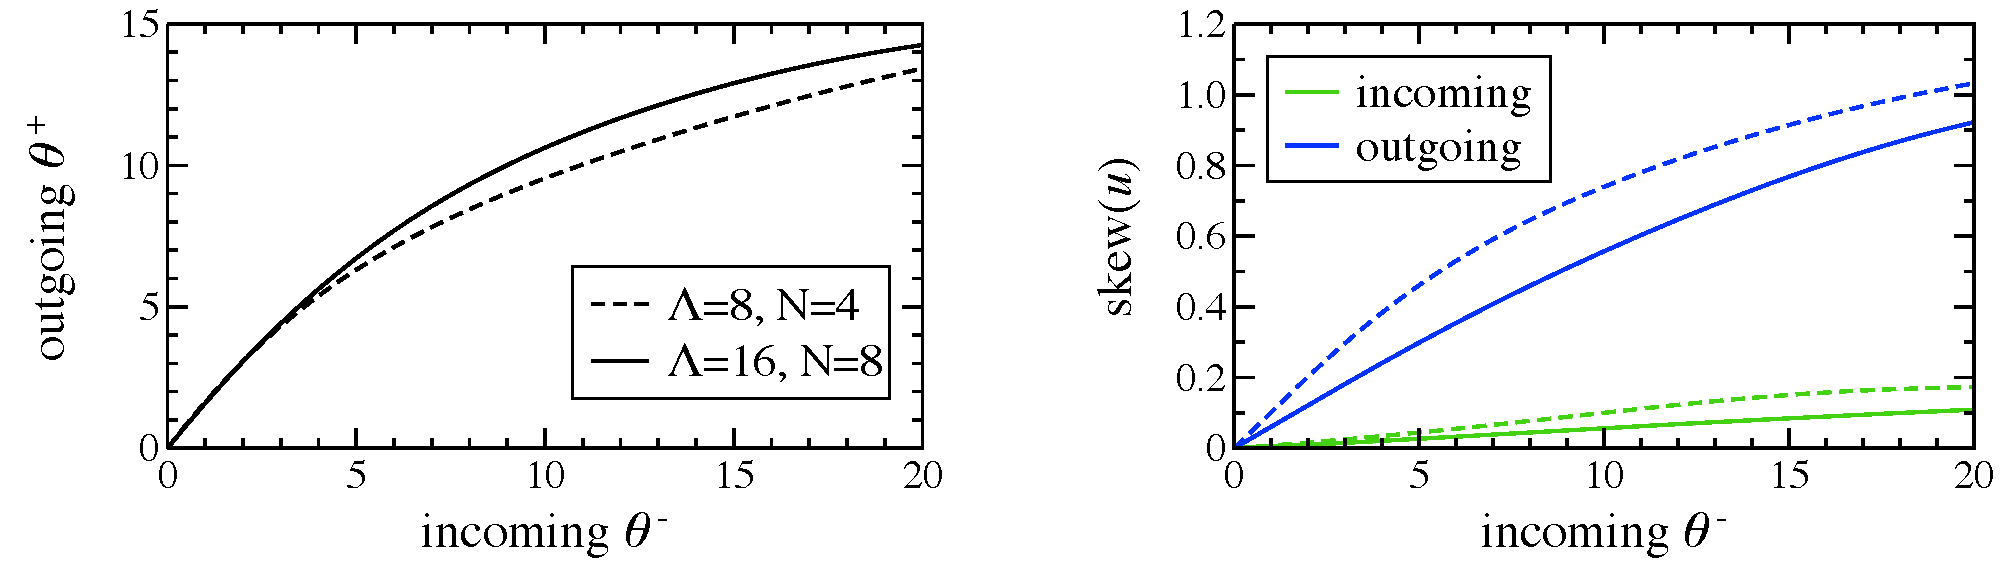
\includegraphics[width = 0.99 \linewidth]{Figs/transfig.pdf}
\caption{
Transfer function
}
\label{transfig}
\end{center}
\end{figure}
 %^^^^^^^^^^^^^^^^^^^^^^^^^^^^^^%

Figure \ref{transfig}(a) shows the transfer function $\thdn = \transf(\thup)$ that results from the statistical matching condition \eqref{statmatch}, for an incoming inverse temperature in the range $\thup \in [0,20]$. In this figure, all model parameters are set by their experimental values, and we show the cases $\Lambda = 8, 16, 32$ with $\lamfac = \Lambda/2$ in each. As seen here, the transfer function is relatively insensitive to the truncation index since all three curves are relatively close to one another. This insensitivity is a consequence of scaling $\lamfac$ with $\Lambda$ appropriately as discussed previously.

\subsection{Statistical comparison between theory and experiments}

Next, Fig.~\ref{transfig}(b) shows the skewness of the incoming (green) and outgoing (blue) wave fields, as they depends on the incoming inverse temperature $\thup$. In line with experimental observations, the incoming skewness is small (always less than 0.2), while the outgoing wave skewness is much higher. Specifically, to capture the experimentally observed peak skewness of about 0.7, we can choose the value of $\thup$ in the range 10--15.

Figure \ref{uhist} shows histograms of the displacement $u$ from experiments and from TKdV theory. The experimental measurements have been normalized for comparison purposes. The comparison is fucking amazing! Offers convincing evidence that the theory works and the parameters have been matched as well as possible. (At some point, I need to mention the minor point about the forcing spectrum not being matched to the Gibbs measure because it came first).

% Figure
%^^^^^^^^^^^^^^^^^^^^^^^^^^^^^^%
\begin{figure}%[!ht]
\begin{center}
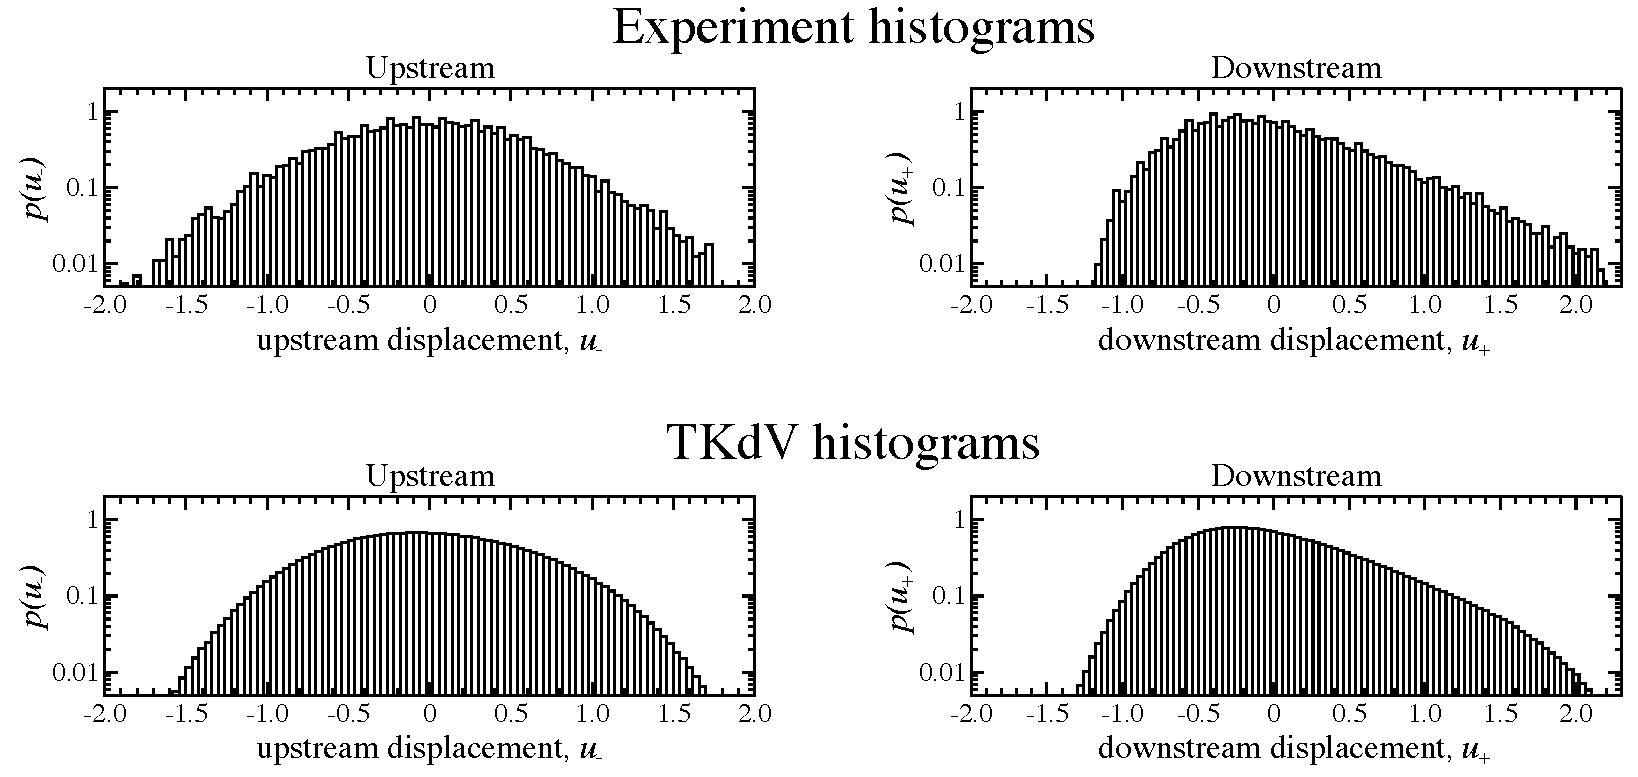
\includegraphics[width = 0.99 \linewidth]{Figs/uhist.pdf}
\caption{
Amazing!
}
\label{uhist}
\end{center}
\end{figure}
 %^^^^^^^^^^^^^^^^^^^^^^^^^^^^^^%
% As of now the simulations use thup=15, thdn=13.

We show histograms of the surface slope in Fig.~\ref{slopehist}, from both the experiments (top) and theory (bottom). The derivative, $\partial \eta / \partial x$, is already a dimensionless quantity with a simple physical interpretation, namely the slope of the free surface, whereas the interpretation of $\partial u/\partial \tilde{x}$ is tied to the characteristic values $\ampscale$ and $\lengthscale$. 
Therefore, in Fig.~\ref{slopehist}, we convert the theoretical calculated values to physical slope via
\begin{equation}
\pd{\eta}{x} = 2 \pi^{3/2} \frac{\etastd}{\lamupdn} \pd{\uupdn}{\tilde{x}}
%\frac{\ampscale \lamfac}{\lengthscale} \pd{\uupdn}{\tilde{x}}
\end{equation}
We have included the $\lamfac$ in the numerator due to the differences in forcing spectra. If the experiments were conducted with the forcing given by the incoming Gibbs measure literally, then there would be no need for $\lamfac$. But the experimental forcing (which was decided before the theory) has a peak frequency of $\freqp = 2 Hz$ and so the factor $\lamfac$ makes $\freqp$ correspond to the dominant value in the spectrum in the theory (REWORD).


% Figure
%^^^^^^^^^^^^^^^^^^^^^^^^^^^^^^%
\begin{figure}%[!ht]
\begin{center}
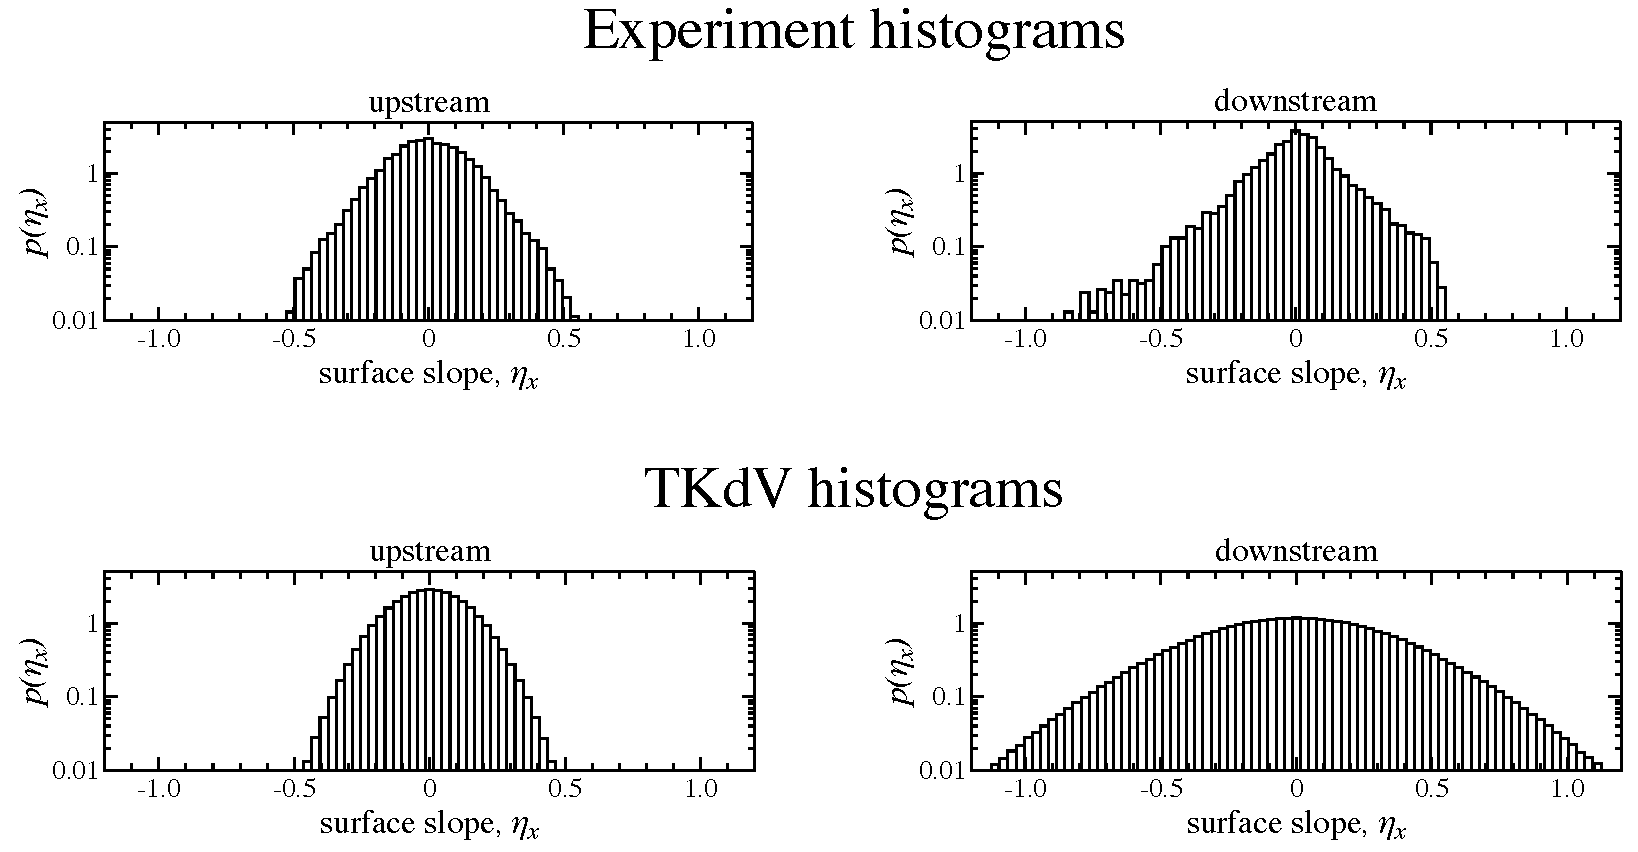
\includegraphics[width = 0.99 \linewidth]{Figs/slopehist.pdf}
\caption{
Slopes
}
\label{slopehist}
\end{center}
\end{figure}
 %^^^^^^^^^^^^^^^^^^^^^^^^^^^^^^%
% As of now the simulations use thup=15, thdn=13.

\subsection{Wave dynamics}

We show individual trajectories in the next figure for upstream and downstream. In the upstream flow, due to the coefficients, the nonlinearity is very weak. Hence, wave propagation is dominated by linear dispersion. Indeed, with weak nonlinearity, \eqref{dimlessKdV} is approximated by
\begin{equation}
u_t + C_2 \drat^{1/2} \, u_{xxx} = 0
\qquad \text{for } x \in [-\pi,\pi] \\
\end{equation}
which implies the dispersion relation $\omega_k = -C_2 k^3$ or for phase velocity $c_k = -C_2 k^2$, which implies left-going waves \cite{majdaqi2019}.
% Further details, see page 6 of Majda Qi, J Stat Phys.

% Figure
%^^^^^^^^^^^^^^^^^^^^^^^^^^^^^^%
\begin{figure}%[!ht]
\begin{center}
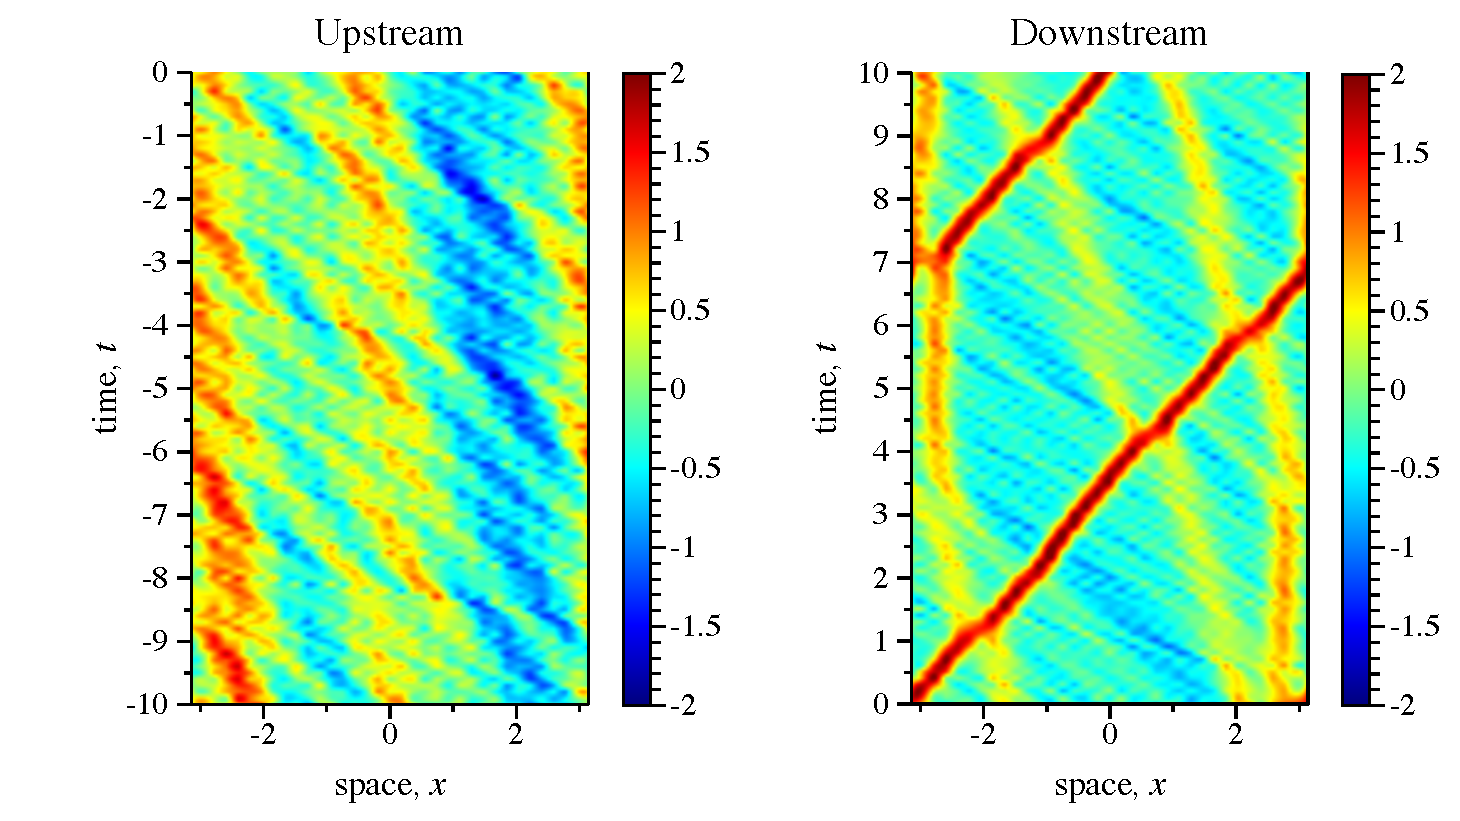
\includegraphics[width = 0.99 \linewidth]{Figs/trajectories.pdf}
\caption{
Trajectories
}
\label{trajectories}
\end{center}
\end{figure}
 %^^^^^^^^^^^^^^^^^^^^^^^^^^^^^^%

% Figure
%^^^^^^^^^^^^^^^^^^^^^^^^^^^^^^%
\begin{figure}%[!ht]
\begin{center}
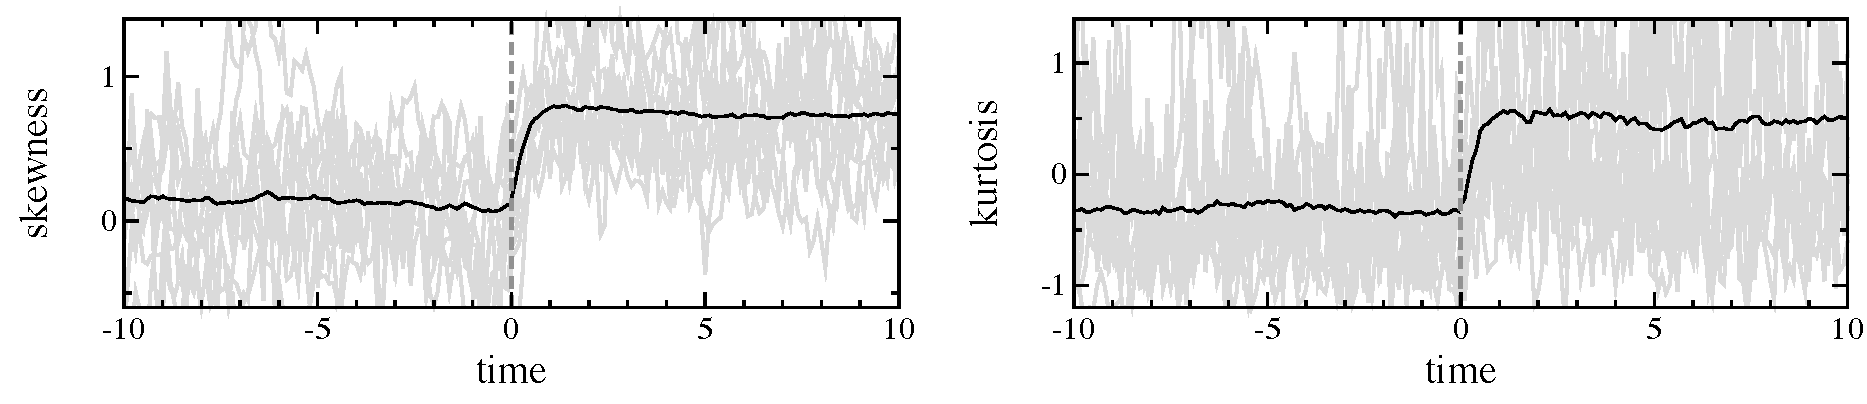
\includegraphics[width = 0.99 \linewidth]{Figs/skew-kurt.pdf}
\caption{
Skewness and kurtosis in DNS}
\label{skew-kurt}
\end{center}
\end{figure}
 %^^^^^^^^^^^^^^^^^^^^^^^^^^^^^^%
 
 
\vsp{5}
%----------------------------------------------------------------------------%
% Skewness formula
%----------------------------------------------------------------------------%
\subsection{Explicit formula for outgoing skewness}
We now examine an explicit formula for the outgoing skewness as originally founded in \cite{majda2019}.
An experimental observation is that the incoming skewness is small, $\meanup{H_3} \approx 0$. Inserting this approximation into the statistical matching condition \eqref{statmatch} and simplifying gives
\begin{equation}
\label{H3H2}
\frac{\meandn{\Hthree^+}} {\meandn{\Htwo^+} - \meanup{\Htwo^+}} = \frac{C_2}{C_3} \dratdn^2
\end{equation}
%where $\Delta \mean{H_2} =  \meandn{H_2} - \meanup{H_2}$  indicates the difference between the upstream and downstream values.
To convert to dimensional, i.e.~experimental, values we first note that
\begin{align}
\mean{\Hthree^+} = \frac{\pi}{3} \mean{u^3} = 
\frac{1}{3} \pi^{-1/2} \frac{\mean{\eta^3}}{\etastd^3} = \frac{1}{3} \pi^{-1/2} \skw(\eta)
\end{align}
Second, to convert the downstream surface slope, we note
\begin{align}
\pd{u}{\tilde{x}} = \frac{\lamfac \lamdn}{\pi^{3/2} \etastd} \pd{\eta}{\xi}
\end{align}
where slope with respect to $\xi$ is the same as with respect to dimensional $x$.
Note: I believe it is important here to use $\lamdn$ in reverting to dimensional variables since we are matching $\Hdn$.
Hence, we have
\begin{align}
&\mean{\Htwo^+} = \pi \mean{ \left( \pd{u}{\tilde{x}} \right)^2} = 
\left( \frac{\lamfac \lamdn}{\pi \etastd} \right)^2 \var(\eta_x)
\end{align}
%
Then algebra gives
\begin{equation}
\frac{\meandn{\Hthree}} {\meandn{\Htwo} - \meanup{\Htwo}} = 
\frac{\pi^{3/2} \, \etastd^2} {3 \lamfac^2 \lamdn^2} 
\left( \frac{\skwdn(\eta)} { \vardn(\eta_x) - \varup(\eta_x)} \right)
\end{equation}
Also we have the simplification
\begin{equation}
\frac{C_2}{C_3} = \frac{\pi^{3/2} \delup^2}{9 \lamfac^2 \epsup}
\end{equation}
Hence, \eqref{H3H2} gives the remarkably explicit formula
\begin{equation}
\frac{\skwdn(\eta)} {\vardn(\eta_x) - \varup(\eta_x)} = \frac{1}{3} \epsup^{-3} \dratdn^3 =
\frac{1}{3} \left( \frac{\ddn}{\etastd} \right)^3
\end{equation}
In particular, the ratio on the left, which can be measured in the experiments, is predicted to scale as the inverse cube of the wave amplitude and as the square of the depth ratio.
% Note: previously I had D^2 on the RHS. The power of 3 comes from using lamdn consistently in the nondimensionalization.






\vsp{10}
%----------------------------------------------------------%
% Direct numerical simulations
%----------------------------------------------------------%
\section{Direct numerical simulations}

\section{Sampling Algorithms}
%\subsection{Naive acceptance-rejection algorithm}
%\subsection{Markov-chain Monte Carlo}
%\subsection{Improved acceptance-rejection algorithm}


%----------------------------------------------------------%
% Comparison with experiments
%----------------------------------------------------------%
\section{Comparison with experiments}

% Figure
%^^^^^^^^^^^^^^^^^^^^^^^^^^^^^^%
\begin{figure}%[!ht]
\begin{center}
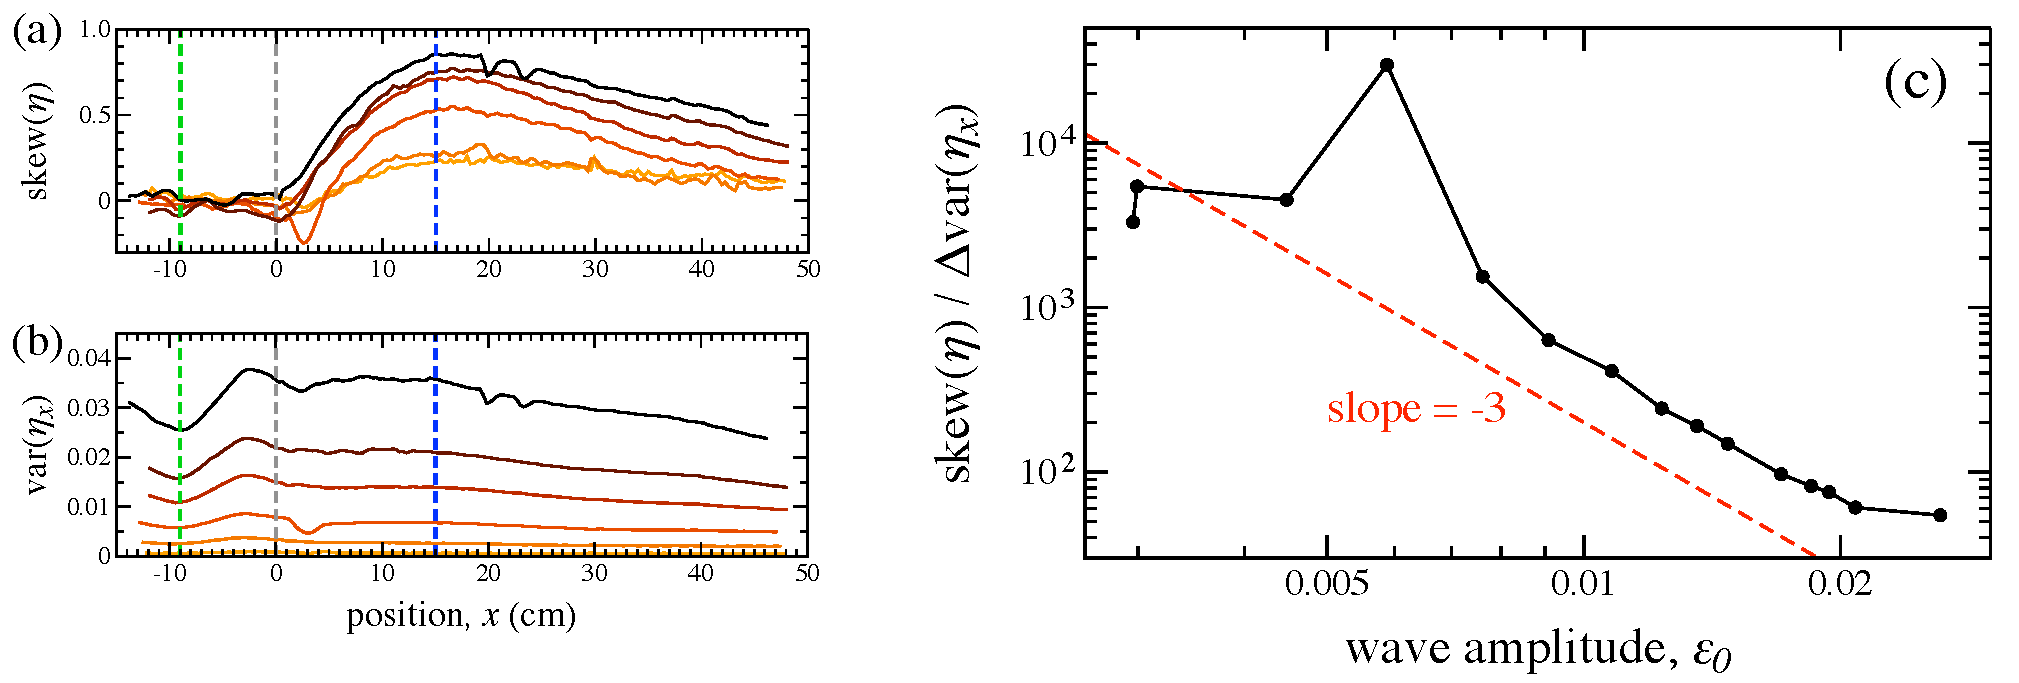
\includegraphics[width = 0.99 \linewidth]{Figs/SkewRat.pdf}
\caption{
Relationship predicted by the theory and confirmed by experiments.
}
\label{AAA}
\end{center}
\end{figure}
 %^^^^^^^^^^^^^^^^^^^^^^^^^^^^^^%
 %New experimental measurements guided by theory

\section*{Acknowledgements}
CTB acknowledges support from the IDEA grant at Florida State University, as well as from the Geophysical Fluid Dynamics Institute. 
MNJM acknowledges support from the Simons Foundation, award 524259. 

\bibliographystyle{plain}
\bibliography{wavesbib}

\end{document}
